\documentclass{ximera}

\input{../../../preamble.tex}


\definecolor{fvdnavy}{HTML}{071D43}
\definecolor{fvdcyan}{HTML}{20BFC6}
\definecolor{fvdcyanlight}{HTML}{EFFCFB}
\definecolor{fvdmagenta}{HTML}{F10D69}
\definecolor{fvdmagentalight}{HTML}{FFF1F7}
\definecolor{fvdtext}{HTML}{163044}





%=================================================
% Pedagogische omgevingen
% PDF: tcolorbox
% HTML: learning-box
%=================================================

\newenvironment{voorkennis}
{%
    \ifdefined\HCode
        \HCode{%
<section class="learning-box learning-box--prior">
<div class="learning-box__header">
<span class="learning-box__icon" aria-hidden="true"></span>
<span class="learning-box__title">Voorkennis</span>
</div>
<div class="learning-box__content">
        }%
        \begin{itemize}
    \else
       \begin{tcolorbox}[
    enhanced,
    breakable,
    colback=fvdcyanlight,
    colframe=fvdcyan,
    coltext=fvdtext,
    boxrule=0.5pt,
    leftrule=4pt,
    arc=4mm,
    outer arc=4mm,
    left=7mm,
    right=6mm,
    top=5mm,
    bottom=5mm,
    before skip=6mm,
    after skip=6mm,
    title=Voorkennis,
    coltitle=fvdcyan,
    fonttitle=\bfseries\Large,
    attach title to upper={\par\smallskip},
    boxed title style={
        empty,
        left=0mm,
        right=0mm,
        top=0mm,
        bottom=0mm
    },
    overlay={
        \draw[
            fvdcyan,
            line width=0.5pt
        ]
        ([xshift=42mm,yshift=-13mm]frame.north west)
        --
        ([xshift=-7mm,yshift=-13mm]frame.north east);
    }
]
        \begin{itemize}
    \fi
}
{%
    \end{itemize}
    \ifdefined\HCode
        \HCode{%
</div>
</section>
        }%
    \else
        \end{tcolorbox}
    \fi
}


\newenvironment{leerdoelen}
{%
    \ifdefined\HCode
        \HCode{%
<section class="learning-box learning-box--goals">
<div class="learning-box__header">
<span class="learning-box__icon" aria-hidden="true"></span>
<span class="learning-box__title">Leerdoelen</span>
</div>
<div class="learning-box__content">
        }%
        \begin{itemize}
    \else
\begin{tcolorbox}[
    enhanced,
    breakable,
    colback=fvdmagentalight,
    colframe=fvdmagenta,
    coltext=fvdtext,
    boxrule=0.5pt,
    leftrule=4pt,
    arc=4mm,
    outer arc=4mm,
    left=7mm,
    right=6mm,
    top=5mm,
    bottom=5mm,
    before skip=6mm,
    after skip=6mm,
    title=Leerdoelen,
    coltitle=fvdmagenta,
    fonttitle=\bfseries\Large,
    attach title to upper={\par\smallskip},
    boxed title style={
        empty,
        left=0mm,
        right=0mm,
        top=0mm,
        bottom=0mm
    },
    overlay={
        \draw[
            fvdmagenta,
            line width=0.5pt
        ]
        ([xshift=42mm,yshift=-13mm]frame.north west)
        --
        ([xshift=-7mm,yshift=-13mm]frame.north east);
    }
]
        \begin{itemize}
    \fi
}
{%
    \end{itemize}
    \ifdefined\HCode
        \HCode{%
</div>
</section>
        }%
    \else
        \end{tcolorbox}
    \fi
}



\title{De inverse functie}
\author{Ingmar Herreman}

\begin{document}

% FVD_CHAPTER_DATA_START
% Automatisch gegenereerd uit index.tex.
% Niet handmatig aanpassen.
\fvdchapterdata{4}{Van relatie naar functie}{4}
% FVD_CHAPTER_DATA_END









\begin{abstract}
In het vorige hoofdstuk onderzochten we wanneer een functie een eenduidige
terugweg heeft. Dat is precies het geval bij een bijectie.

Nu construeren we die terugweg. We leren wat een \textbf{inverse functie} is,
hoe domein en bereik van plaats wisselen, hoe we een eenvoudig voorschrift
van een inverse bepalen en vooral hoe de grafieken van een functie en haar
inverse met elkaar samenhangen.

De centrale grafische ontdekking is dat beide grafieken elkaars spiegelbeeld
zijn ten opzichte van de rechte
\[
y=x.
\]
\end{abstract}

\maketitle

\begin{voorkennis}
    \item Je begrijpt domein, codomein en bereik.
    \item Je kan beelden en originelen bepalen.
    \item Je begrijpt injectiviteit, surjectiviteit en bijectiviteit.
    \item Je kan met de horizontale-lijntest onderzoeken of een functie injectief is.
    \item Je begrijpt waarom een bijectie een eenduidige terugweg heeft.
\end{voorkennis}

\begin{leerdoelen}
    \item Je kan uitleggen wat de inverse functie van een bijectie betekent.
    \item Je kan \(f^{-1}\) correct interpreteren en onderscheiden van \(\frac1f\).
    \item Je kan het verband tussen domein en bereik van \(f\) en \(f^{-1}\) uitleggen.
    \item Je kan grafisch verklaren waarom de grafieken van \(f\) en \(f^{-1}\)
          elkaars spiegelbeeld zijn ten opzichte van \(y=x\).
    \item Je kan vanuit een grafiek de inverse grafiek construeren en analyseren.
    \item Je kan bij eenvoudige functies algebraïsch een voorschrift van de inverse bepalen.
    \item Je kan een gevonden inverse controleren door heen-en-terug te gaan.
    \item Je kan in een context uitleggen wat het omkeren van een functie betekent.
    \item Je kan GeoGebra gebruiken om het verband tussen een functie en haar inverse te onderzoeken.
\end{leerdoelen}



% ============================================================
% 1. DE TERUGWEG
% ============================================================

\FVDsection{De terugweg van een functie}

Beschouw de bijectie
\[
f:\mathbb R\to\mathbb R:x\mapsto 2x+3.
\]

De functie stuurt bijvoorbeeld
\[
4\longmapsto 11.
\]

Omdat \(f\) bijectief is, heeft \(11\) precies één origineel.
De terugweg stuurt dus
\[
11\longmapsto4.
\]

Die terugweg noemen we de \textbf{inverse functie}.

\begin{definitie}
Als \(f:A\to B\) een bijectie is, dan is de \textbf{inverse functie}
\[
f^{-1}:B\to A
\]
de functie die ieder element \(y\in B\) terugstuurt naar zijn unieke origineel
door \(f\).

Dus:
\[
f(x)=y
\quad\Longleftrightarrow\quad
f^{-1}(y)=x.
\]
\end{definitie}

\begin{center}
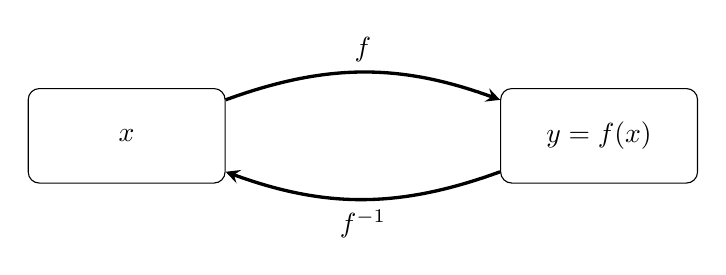
\begin{tikzpicture}[>=stealth]
\node[draw,rounded corners,minimum width=2.5cm,minimum height=1.2cm] (A) at (-3,0) {$x$};
\node[draw,rounded corners,minimum width=2.5cm,minimum height=1.2cm] (B) at (3,0) {$y=f(x)$};
\draw[->,very thick,bend left=20] (A) to node[above] {$f$} (B);
\draw[->,very thick,bend left=20] (B) to node[below] {$f^{-1}$} (A);
\end{tikzpicture}
\end{center}

\begin{opmerking}[Belangrijke notatie]
De notatie
\[
f^{-1}
\]
betekent \textbf{inverse functie}.

Ze betekent niet
\[
\frac{1}{f}.
\]

In het algemeen geldt dus
\[
\boxed{f^{-1}(x)\neq\frac{1}{f(x)}.}
\]
\end{opmerking}

% ============================================================
% 2. DOMEIN EN BEREIK WISSELEN
% ============================================================

\FVDsection{Domein en bereik wisselen van rol}

Als
\[
f:A\to B
\]
bijectief is, dan loopt de inverse functie in de andere richting:
\[
f^{-1}:B\to A.
\]

Daarom wisselen domein en bereik van rol.

\begin{eigenschap}
Voor een inverteerbare functie \(f\):
\[
\boxed{\operatorname{dom}f^{-1}=\operatorname{ber}f}
\]
en
\[
\boxed{\operatorname{ber}f^{-1}=\operatorname{dom}f.}
\]
\end{eigenschap}

\begin{voorbeeld}
Beschouw
\[
f:[0,+\infty[\to[1,+\infty[:x\mapsto x^2+1.
\]

Dan
\[
\operatorname{dom}f=[0,+\infty[
\]
en
\[
\operatorname{ber}f=[1,+\infty[.
\]

De inverse zal daarom voldoen aan
\[
\operatorname{dom}f^{-1}=[1,+\infty[
\]
en
\[
\operatorname{ber}f^{-1}=[0,+\infty[.
\]
\end{voorbeeld}

% ============================================================
% 3. PUNTEN WISSELEN VAN COÖRDINATEN
% ============================================================

\FVDsection{Wat gebeurt er met punten op de grafiek?}

Stel dat
\[
f(a)=b.
\]

Dan ligt
\[
(a,b)
\]
op de grafiek van \(f\).

Omdat
\[
f^{-1}(b)=a,
\]
ligt
\[
(b,a)
\]
op de grafiek van \(f^{-1}\).

Dus:

\[
\boxed{(a,b)\text{ op }f\quad\Longleftrightarrow\quad(b,a)\text{ op }f^{-1}.}
\]

\begin{center}
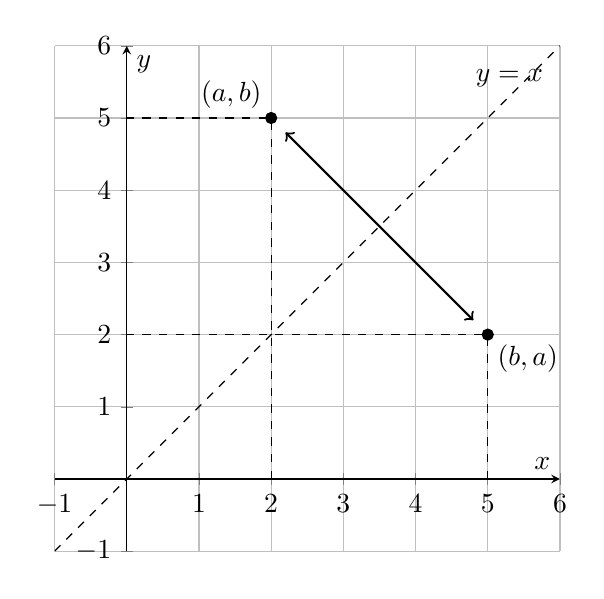
\begin{tikzpicture}
\begin{axis}[
    width=9cm,height=8cm,
    xmin=-1,xmax=6,ymin=-1,ymax=6,
    xlabel={$x$},ylabel={$y$},
    axis lines=middle,grid=both,
    axis equal image
]
\addplot[dashed,domain=-1:6] {x};
\addplot[only marks,mark=*] coordinates {(2,5)(5,2)};
\draw[dashed] (axis cs:2,0)--(axis cs:2,5)--(axis cs:0,5);
\draw[dashed] (axis cs:5,0)--(axis cs:5,2)--(axis cs:0,2);
\draw[<->,thick] (axis cs:2.2,4.8)--(axis cs:4.8,2.2);
\node[above left] at (axis cs:2,5) {$(a,b)$};
\node[below right] at (axis cs:5,2) {$(b,a)$};
\node[above] at (axis cs:5.3,5.3) {$y=x$};
\end{axis}
\end{tikzpicture}
\end{center}

Het verwisselen van de coördinaten
\[
(a,b)\longleftrightarrow(b,a)
\]
is precies een spiegeling ten opzichte van de rechte \(y=x\).

% ============================================================
% 4. GRAFISCH VERBAND
% ============================================================

\FVDsection{De grafieken van \(f\) en \(f^{-1}\)}

We komen bij het centrale grafische resultaat.

\begin{eigenschap}
De grafiek van een inverteerbare functie \(f\) en de grafiek van haar inverse
\(f^{-1}\) zijn elkaars spiegelbeeld ten opzichte van
\[
\boxed{y=x.}
\]
\end{eigenschap}

\begin{voorbeeld}[Een lineaire functie en haar inverse]

Neem
\[
f(x)=2x+1.
\]

De inverse functie is
\[
f^{-1}(x)=\frac{x-1}{2}.
\]

\begin{center}
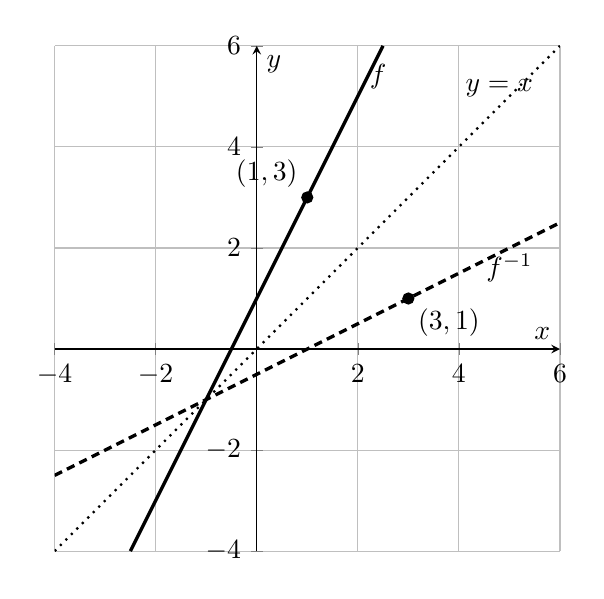
\begin{tikzpicture}
\begin{axis}[
    width=10cm,height=8cm,
    xmin=-4,xmax=6,ymin=-4,ymax=6,
    xlabel={$x$},ylabel={$y$},
    axis lines=middle,grid=both,
    axis equal image,
    samples=120
]
\addplot[very thick,domain=-2.5:2.5] {2*x+1};
\addplot[very thick,densely dashed,domain=-4:6] {(x-1)/2};
\addplot[dotted,thick,domain=-4:6] {x};
\addplot[only marks,mark=*] coordinates {(1,3)(3,1)};
\node[above left] at (axis cs:1,3) {$(1,3)$};
\node[below right] at (axis cs:3,1) {$(3,1)$};
\node at (axis cs:2.4,5.4) {$f$};
\node at (axis cs:5,1.6) {$f^{-1}$};
\node[above] at (axis cs:4.8,4.8) {$y=x$};
\end{axis}
\end{tikzpicture}
\end{center}

Het punt \((1,3)\) op \(f\) wordt door spiegeling in \(y=x\)
het punt \((3,1)\) op \(f^{-1}\).
\end{voorbeeld}

\begin{opmerking}
Het is niet voldoende om de regel ``spiegelen in \(y=x\)'' uit het hoofd
te leren. Je moet kunnen verklaren \emph{waarom} ze geldt:

\[
f(a)=b
\Longleftrightarrow
f^{-1}(b)=a
\Longleftrightarrow
(a,b)\leftrightarrow(b,a).
\]
\end{opmerking}

% ============================================================
% 5. GRAFISCH CONSTRUEREN
% ============================================================

\FVDsection{Een inverse grafiek construeren}

Als de grafiek van een bijectieve functie gegeven is, kunnen we de inverse
grafiek construeren zonder een voorschrift te kennen.

\begin{enumerate}
    \item Teken de rechte \(y=x\).
    \item Kies herkenbare punten op de grafiek van \(f\).
    \item Verwissel bij elk punt de coördinaten:
    \[
    (a,b)\mapsto(b,a).
    \]
    \item Spiegel de volledige grafiek in \(y=x\).
\end{enumerate}

\begin{voorbeeld}[Inverse zonder voorschrift]

Stel dat een functie door de punten
\[
(-2,-1),\quad(0,1),\quad(1,3),\quad(3,4)
\]
loopt en tussen deze punten strikt stijgt.

Dan loopt de inverse grafiek door
\[
(-1,-2),\quad(1,0),\quad(3,1),\quad(4,3).
\]

\begin{center}
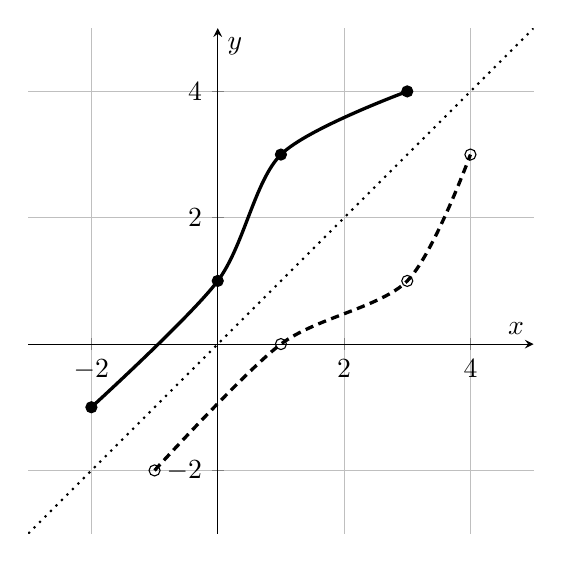
\begin{tikzpicture}
\begin{axis}[
    width=10cm,height=8cm,
    xmin=-3,xmax=5,ymin=-3,ymax=5,
    xlabel={$x$},ylabel={$y$},
    axis lines=middle,grid=both,
    axis equal image
]
\addplot[very thick,smooth] coordinates {(-2,-1)(0,1)(1,3)(3,4)};
\addplot[very thick,densely dashed,smooth] coordinates {(-1,-2)(1,0)(3,1)(4,3)};
\addplot[dotted,thick,domain=-3:5] {x};
\addplot[only marks,mark=*] coordinates {(-2,-1)(0,1)(1,3)(3,4)};
\addplot[only marks,mark=o] coordinates {(-1,-2)(1,0)(3,1)(4,3)};
\end{axis}
\end{tikzpicture}
\end{center}
\end{voorbeeld}

% ============================================================
% 6. VOORSCHRIFT BEPALEN
% ============================================================

\FVDsection{Het voorschrift van de inverse bepalen}

Bij eenvoudige functies kunnen we het inverse voorschrift algebraïsch bepalen.

Vertrek van
\[
y=f(x).
\]

Omdat de inverse invoer en uitvoer verwisselt, wisselen we \(x\) en \(y\)
en lossen daarna op naar \(y\).

\begin{voorbeeld}[Lineaire functie]

Gegeven
\[
f(x)=3x-5.
\]

Schrijf
\[
y=3x-5.
\]

Verwissel \(x\) en \(y\):
\[
x=3y-5.
\]

Los op naar \(y\):
\[
3y=x+5,
\]
dus
\[
y=\frac{x+5}{3}.
\]

Daarom
\[
\boxed{f^{-1}(x)=\frac{x+5}{3}.}
\]
\end{voorbeeld}

\begin{voorbeeld}[Kwadraatfunctie met domeinbeperking]

Beschouw
\[
f:[0,+\infty[\to[1,+\infty[:x\mapsto x^2+1.
\]

De domeinbeperking is essentieel: zonder die beperking zou \(f\) niet
injectief zijn.

Vertrek van
\[
y=x^2+1.
\]

Verwissel:
\[
x=y^2+1.
\]

Dan
\[
y^2=x-1.
\]

Omdat het bereik van de inverse gelijk is aan het oorspronkelijke domein
\([0,+\infty[\), kiezen we de niet-negatieve wortel:
\[
\boxed{f^{-1}(x)=\sqrt{x-1}.}
\]

Hierbij
\[
\operatorname{dom}f^{-1}=[1,+\infty[.
\]
\end{voorbeeld}

\begin{opmerking}
Het teken bij een wortel kies je niet willekeurig. Het wordt bepaald door
het domein dat voor de oorspronkelijke functie gekozen werd.

Voor
\[
f:]-\infty,0]\to[0,+\infty[:x\mapsto x^2
\]
zou de inverse bijvoorbeeld
\[
f^{-1}(x)=-\sqrt{x}
\]
zijn.
\end{opmerking}

% ============================================================
% 7. CONTROLEREN DOOR HEEN EN TERUG
% ============================================================

\FVDsection{Controleren: heen en terug}

Als twee functies werkelijk elkaars inverse zijn, dan brengt eerst de ene
en daarna de andere functie ons terug naar de beginwaarde.

\begin{eigenschap}
Voor passende waarden geldt
\[
\boxed{f^{-1}(f(x))=x}
\]
en
\[
\boxed{f(f^{-1}(x))=x.}
\]
\end{eigenschap}

\begin{voorbeeld}
Neem
\[
f(x)=2x+3
\qquad\text{en}\qquad
f^{-1}(x)=\frac{x-3}{2}.
\]

Dan
\[
f^{-1}(f(x))
=
\frac{(2x+3)-3}{2}
=
x.
\]

Ook:
\[
f(f^{-1}(x))
=
2\left(\frac{x-3}{2}\right)+3
=
x.
\]

De twee functies maken elkaars werking ongedaan.
\end{voorbeeld}

\begin{opmerking}[Vooruitblik naar samengestelde functies]
In de bovenstaande controle voeren we twee functies na elkaar uit.
Dat is een voorbeeld van een \textbf{samengestelde functie}.

We gebruiken dit begrip hier alleen functioneel om inversen te controleren.
Later bouwen we samengestelde functies systematischer op, omdat ze onder
andere noodzakelijk zijn voor de kettingregel bij afgeleiden.
\end{opmerking}

% ============================================================
% 8. GEOGEBRA
% ============================================================

\FVDsection{De inverse onderzoeken met GeoGebra}

\begin{opmerking}[GeoGebra-onderzoek: spiegeling in \(y=x\)]
Voer in GeoGebra bijvoorbeeld
\[
f(x)=2x+1
\]
in en teken ook
\[
y=x.
\]

Voer daarna de inverse functie in:
\[
g(x)=\frac{x-1}{2}.
\]

Onderzoek:

\begin{enumerate}
    \item Kies een punt \(A\) op de grafiek van \(f\).
    \item Spiegel \(A\) in de rechte \(y=x\).
    \item Ligt het spiegelbeeld op de grafiek van \(g\)?
    \item Herhaal dit voor verschillende punten.
    \item Vergelijk domein en bereik van beide functies.
\end{enumerate}

Herhaal daarna het onderzoek met
\[
f(x)=x^2+1,\qquad x\geq0,
\]
en
\[
f^{-1}(x)=\sqrt{x-1}.
\]

Formuleer op basis van je waarnemingen zelf het grafische verband tussen
een functie en haar inverse.
\end{opmerking}

% ============================================================
% 9. CONTEXT
% ============================================================

\FVDsection{Inverse functies in een STEM-context}

Een inverse functie heeft een natuurlijke betekenis wanneer een meet- of
omzettingsproces moet worden teruggedraaid.

\begin{voorbeeld}[Temperatuursensor kalibreren]

Een temperatuursensor heeft in zijn werkgebied het model
\[
U(T)=0{,}50+0{,}020T,
\qquad -20\leq T\leq80.
\]

De functie zet temperatuur om in spanning:
\[
T\longmapsto U.
\]

In een meettoestel gebeurt juist het omgekeerde: we meten een spanning en
willen daaruit de temperatuur bepalen.

Vertrek van
\[
U=0{,}50+0{,}020T.
\]

Los op naar \(T\):
\[
T=\frac{U-0{,}50}{0{,}020}.
\]

De inverse functie is dus
\[
\boxed{T(U)=\frac{U-0{,}50}{0{,}020}.}
\]

Voor \(U=1{,}50\) V:
\[
T(1{,}50)=50.
\]

Een spanning van \(1{,}50\) V wordt door het gekalibreerde meetsysteem
dus geïnterpreteerd als \(50^\circ\mathrm C\).

\begin{center}
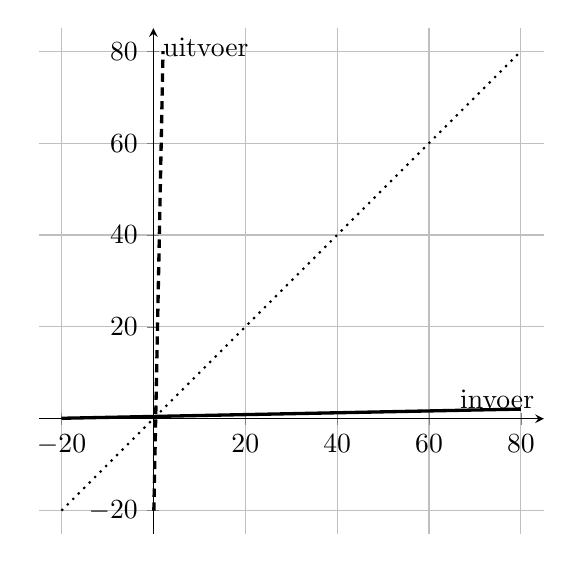
\begin{tikzpicture}
\begin{axis}[
    width=10cm,height=8cm,
    xmin=-25,xmax=85,
    ymin=-25,ymax=85,
    xlabel={invoer},ylabel={uitvoer},
    axis lines=middle,grid=both,
    axis equal image,
    samples=120
]
% herschaalde conceptuele voorstelling om spiegeling zichtbaar te houden
\addplot[very thick,domain=-20:80] {0.5+0.02*x};
\addplot[very thick,densely dashed,domain=0.1:2.1] {(x-0.5)/0.02};
\addplot[dotted,thick,domain=-20:80] {x};
\end{axis}
\end{tikzpicture}
\end{center}

De grafische spiegeling is wiskundig correct, maar in een fysische grafiek
moeten we ook op de \textbf{eenheden van beide assen} letten. Bij het omkeren
wisselen de rollen van temperatuur en spanning.
\end{voorbeeld}

% ============================================================
% 10. WAT ALS DE FUNCTIE NIET BIJECTIEF IS?
% ============================================================

\FVDsection{Wat als de functie niet bijectief is?}

Beschouw opnieuw
\[
f:\mathbb R\to[0,+\infty[:x\mapsto x^2.
\]

Als we de koppels omkeren, krijgen we
\[
y=\pm\sqrt{x}.
\]

Dat is geen functie: een positieve invoer zou twee uitvoerwaarden hebben.

\begin{center}
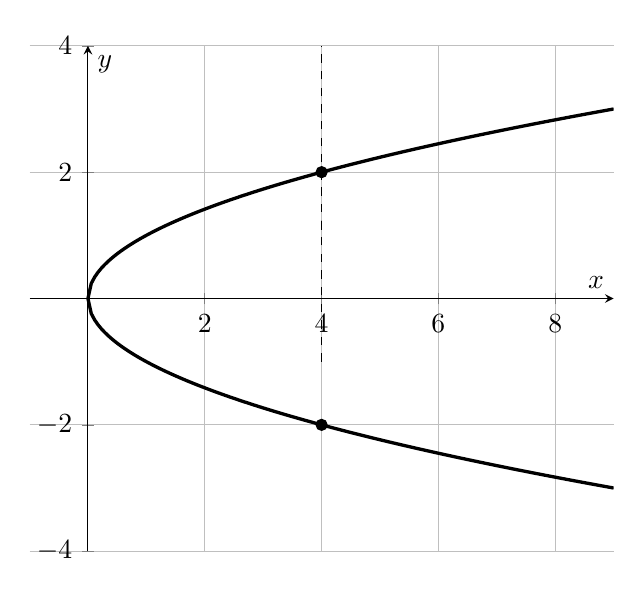
\begin{tikzpicture}
\begin{axis}[
    width=9cm,height=8cm,
    xmin=-1,xmax=9,ymin=-4,ymax=4,
    xlabel={$x$},ylabel={$y$},
    axis lines=middle,grid=both,
    samples=160
]
\addplot[very thick,domain=0:9] {sqrt(x)};
\addplot[very thick,domain=0:9] {-sqrt(x)};
\addplot[dashed,domain=-1:4] ({4},x);
\addplot[only marks,mark=*] coordinates {(4,2)(4,-2)};
\end{axis}
\end{tikzpicture}
\end{center}

De inverse \emph{relatie} bestaat wel, maar ze is geen inverse \emph{functie}.

Na de domeinbeperking
\[
f:[0,+\infty[\to[0,+\infty[:x\mapsto x^2
\]
verdwijnt dit probleem en krijgen we
\[
f^{-1}(x)=\sqrt{x}.
\]

Dit toont opnieuw waarom bijectiviteit geen technisch detail is, maar precies
de voorwaarde die een inverse functie mogelijk maakt.



\end{document}
